\documentclass{article}

% Packages goes here
% snytax \usepackage{amsmath}
\usepackage {lipsum}
\usepackage{todonotes}

\usepackage{graphicx}
\graphicspath{ {images/} }



\begin{document}

	% Make the title page here
	\begin{titlepage}
		\begin{center}
			\line(1,0){300}\\
			\huge{\bfseries Automatic Android Malware Analysis}\\
			\line(1,0){300}\\
		\end{center}
	\end{titlepage}
	
	\tableofcontents
	\cleardoublepage
	
	\section{Introduction}\label{sec:intro}
		\subsection{APK file}\label{sec:apk}	
				\paragraph{} Android Application Package(APK) is the file format used for an android application. It contains all the resources required for an application to run on android operating system. Its basically a zip file or a jar file with extension of ".apk"\cite{APK_structure}.
			\subsubsection{APK file contents}
				\paragraph{} Normally an apk file contains following files or folders:
				
				\todo{Add captions and made the picture available in list of figures}
				\begin{figure}[h]
					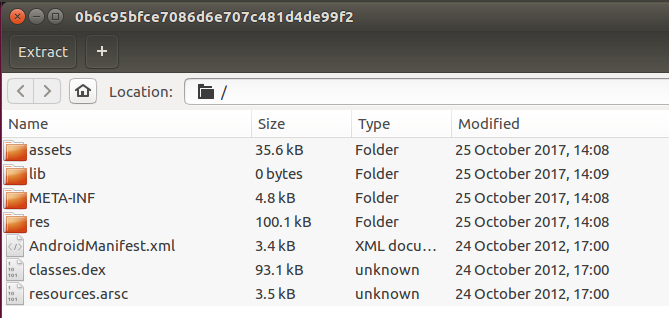
\includegraphics[width=\textwidth]{apk_contents.png}
				\end{figure}

				\begin{itemize}
					\item \textbf{assets/:} It provides a way to include arbitrary files like text, xml, fonts, music and video in your application and allow you to access your data raw/untouched. AssetManager is used to read this data\cite{android_assets}. Due to raw access sometimes this directory contains executable payloads and dynamically loaded code. One interesting usage is storing Dex files in it to avoid its reverse engineering. \cite{lim2016android}
					
					\item \textbf{lib/:} This directory is for natively compiled code. This directory contains a subdirectory for each platform type, like armeabi, armeabi-v7a, arm64-v8a, x86, x86\textunderscore64, and mips \cite{APK_structure}. This code is run directly on CPU and have access to android API using Java Native Interface(JNI). Natively compiled code is more suitable for CPU intensive jobs because of less overhead and good performance of programming language like c/c++. Most of the android  static analysis tools work on Java level- that is, they process either the decompiled Java source code or Dalvik Byte Code\cite{afonso2016going}. This rises several interesting scenarios in which malware authors can avoid detection, can redistributing benign applications with malicious injections or completely modifying behavior of an application. Readers interested in this topic are encouraged to have a look at \cite{afonso2016going}. Android NDK can be used to compile native code for android. \todo{compile hello world in c for android in apendix}


					\item \textbf{META-INF/:} This directory contains the following three files:
					\begin{enumerate}
						\item \textbf{MANIFEST.MF:} Its a text file and contains a list and base64 encoded SHA-1 hashes of all files included in the APK.
						\item \textbf{CERT.SF:} This file again contain a list of all files but this time with the base64 encoded SHA-1 hashes of the corresponding lines in the MANIFEST.MF file. It also contain based64 encoded SHA-1 hash of MANIFEST.MF file.
						\item \textbf{CERT.RSA:} It contains developers public signature, used for validation of upgrades. Its basically singed content of CERT.SF file along with public key to validate the contents.
					\end{enumerate}
					
					\item \textbf{res/:} This directory contain resource which are not compiled into "resources.arsc" (see below) \cite{APK_structure}. These resources can be accessed from inside the application code using resource ID. All resource IDs are defined in "R" class of the project. Application developers can specify alternate resources to support specific device configurations e.g, alternative drawable resources for different screen sizes, alternative strings for different languages etc.

					\item \textbf{AndroidManifest.xml:} Every application must have an AndroidManifest.xml file. This file provide essential information about the application like entry points, package name, components, permissions, minimum level of Android API, libraries, intents etc. For static analysis purposes a lot of information can be extracted from this file.

					\item \textbf{classes.dex:} This is the most important file insude an apk. It contains classes compiled in the DEX file format which can be understood by the Dalvik/ART virtual machine \cite{APK_structure}. In the next section we will describe this file in more details.

					\item \textbf{resources.arsc:} This file contain compiled resources. This file contains the XML content from all configurations of the res/values/ folder. The packaging tool extracts this XML content, compiles it to binary form, and archives the content. This content includes language strings and styles, as well as paths to content that is not included directly in the resources.arsc file, such as layout files and images \cite{APK_structure}. These resources can also be accessed using the "R" class.
				\end{itemize}
		\subsection{Dex file format}\label{sec:dex}				
				\todo{structure of Dex file}
				\lipsum[1]
				
				
				\todo{TODO: Write introduction section after the significant part of report is done and the structure is more clear}
		\lipsum[1]
		\todo{Discuss static analysis and dynamic analysis}
		To be done later, In this chapter we include the problem statement, See fh kiel project report structure for missing parts. Here goes some lipsum
		\lipsum[1]
		
		\pagebreak
		
	\section{Static Analysis}\label{sec:static_analysis}
		There are several static analysis tools available for APKs, each one having its own strengths and weaknesses.
		\todo{Add some info about common tools}
	
		
		\lipsum[1]
			\subsection{Apktool}\label{sec:apktool}
			APKTool is one of the major reverse engineering tool for android applications.  \todo{Add more info}
			\lipsum[2]
			\subsection{Androguard}\label{sec:androguard}
			\todo{Introduce androguard}
			Androguard is an open source tool written in python for analyzing android applications. Its been in a several of tools including Virustotal and Cuckoodroid among others. It can process APK files, dex files or odex files. It can disassemble Dex/Odex files to smali code and can decompile Dex/Odex to Java code. The classes in androguard can be generally divided into two categories: Classes used for parsing and the analysis classes. We will go into more details about these classes but first we will show some basic usage of androguard.
			

			
			\todo{TODO: Do androguard basic usage examples}
			\lipsum[1]
			\todo{Discuss the changes we made including normalization, canonical hasing for similarity search}
			\lipsum[1]
			\todo{Discuss the info we are extracting from apks for platform}
			\lipsum[1]
			\todo{TODO: Do androguard comparison apks to see how many functions has added and how many removed, make a
			table out of it}
			\lipsum[1]
			\todo{TODO: Find reused code section in sonicspy or bankbots or lokibot}
			\lipsum[1]
			\todo{Usage of androguard for extracting features for AI/ML, prepare for talk in AIOLI-FFM group}
			\lipsum[1]
			\todo{Ask lukas for some results from platform}
			\lipsum[1]
			\todo{Improvements in androguard}
			\lipsum[1]
			\pagebreak
	\section{Dynamic Analysis: Cuckoodroid based on Cuckoo sandbox}\label{sec:cuckoodroid}
		
		\todo{Introduction to cuckoodroid}
		\lipsum[1]
		\todo{Fixing cuckoodroid}
		\lipsum[1]
		\todo{Persistent root problem}
		\lipsum[1]
		\todo{Lates android}
		\lipsum[1]
		\todo{python compilation workaround, termux}
		\lipsum[1]
		\todo{Slow android emulator}
		\lipsum[1]
		\pagebreak
	
	\section{Dynamic Analysis: Anti-Emulator Detection}
		\todo{Common methods employed for emulator detection, some literature}
		\lipsum[1]
		\todo{Good and bad uses of anti-emulator detection}
		\lipsum[1]
		\todo{Testing results of cuckoodroid against common emulator detection methods}
		\lipsum[1]
		\todo{Adding some new anti-emulator detection features to cuckoodroid}
		\lipsum[1]
		\todo{result of analysis before and after} 
		\lipsum[1]
		\pagebreak
	
	\bibliographystyle{ieeetr}
	\bibliography{References}
\end{document}